\section{Practical part}
\phantomsection

\subsection{Differences and Similarities between MSSQL and Oracle}
Since MSSQL was base SQL Database for my course work, here I will define things that are different in SQL Database.

\subsubsection{Execution plan}
In SQL Developer to show execution plan, you should press F10 or click the Explain Plan icon. Of course it looks different and has it's features which makes him different of what we have in SSMS.

\begin{figure}[ht!]
	\centering
	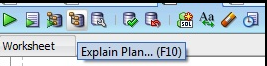
\includegraphics[width=0.4\textwidth]{sqldeveloper_execution_plan}
	\caption{Showing execution plan}
\end{figure}

\subsubsection{Changes index creation queries}
Because Oracle SQL doesn't have \textbf{INCLUDE} statement on creating indexes. To migrate our queries we need only to change queries which have \textbf{INCLUDE} statement.

\lstinputlisting[style=mystyle, language=SQL, caption={Finding product with a given id}]{sourcecode/migration.sql}

\clearpage